%%%%%%%%%%%%%%%%%%%%%%%%%%%%%%%%%%%%%%%%%%%%%%%%%%%%%%%%%%%%%%%%%%%%%%%%%%%%%%%%%%
\begin{frame}[fragile]\frametitle{}
\begin{center}
{\Large Concepts}
\end{center}
\end{frame}

%%%%%%%%%%%%%%%%%%%%%%%%%%%%%%%%%%%%%%%%%%%%%%%%%%%%%%%%%%%
\begin{frame}[fragile]\frametitle{High-Dimensional Representation}
    \begin{itemize}
        \item A 2D point is represented by two values (x, y). They can also be represented by two boxes. First box's black-ness depends on x coordinate and 2nd box's with y coordinate. 0 value means white, 1 means black. 
        \item A 16D point is represented using 16 coordinate values, thus 14 boxes, but can be arranged as 4x4 grid or image.
    \end{itemize}
	
\begin{center}
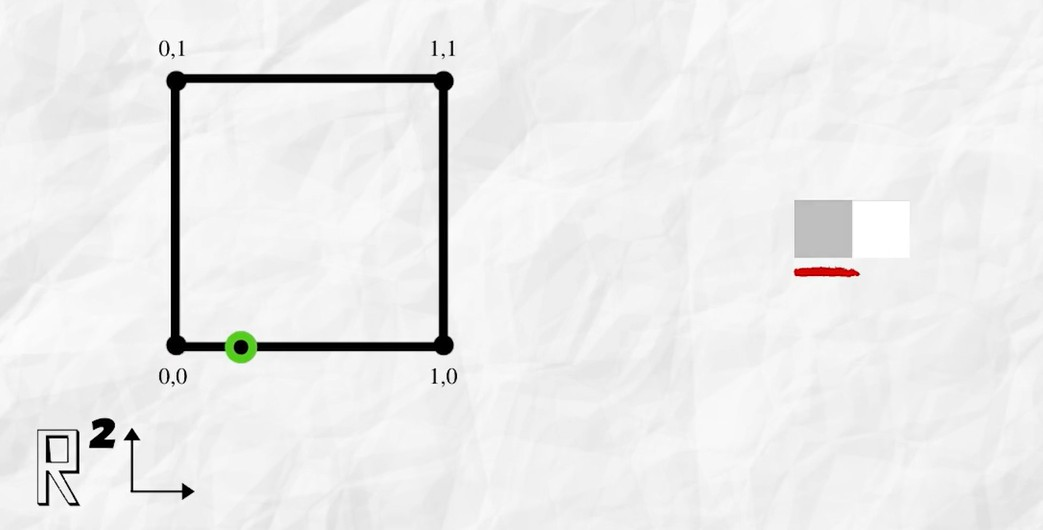
\includegraphics[width=0.45\linewidth,keepaspectratio]{gdl17}
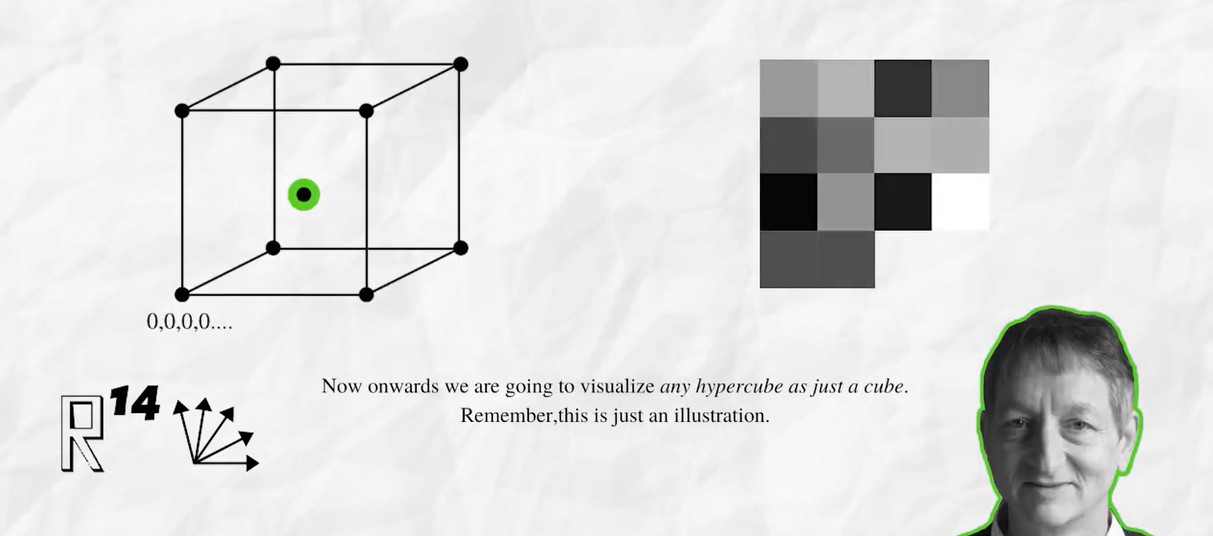
\includegraphics[width=0.45\linewidth,keepaspectratio]{gdl18}

{\tiny (Ref: My Understanding of the Manifold Hypothesis - Kartik Chincholikar)}	

\end{center}

\end{frame}

%%%%%%%%%%%%%%%%%%%%%%%%%%%%%%%%%%%%%%%%%%%%%%%%%%%%%%%%%%%
\begin{frame}[fragile]\frametitle{Images as Points in a Hypercube}
    \begin{itemize}
        \item A grayscale image = point in a high-dimensional space.
        \item 256×256 images, each pixel is a dimension.
        \item All images are just rare points in this vast space.
        \item Random points mostly lead to noise, not meaningful images.
		\item So, only some points in this high dimensional (hyper) space are valid images.
    \end{itemize}
	
\begin{center}
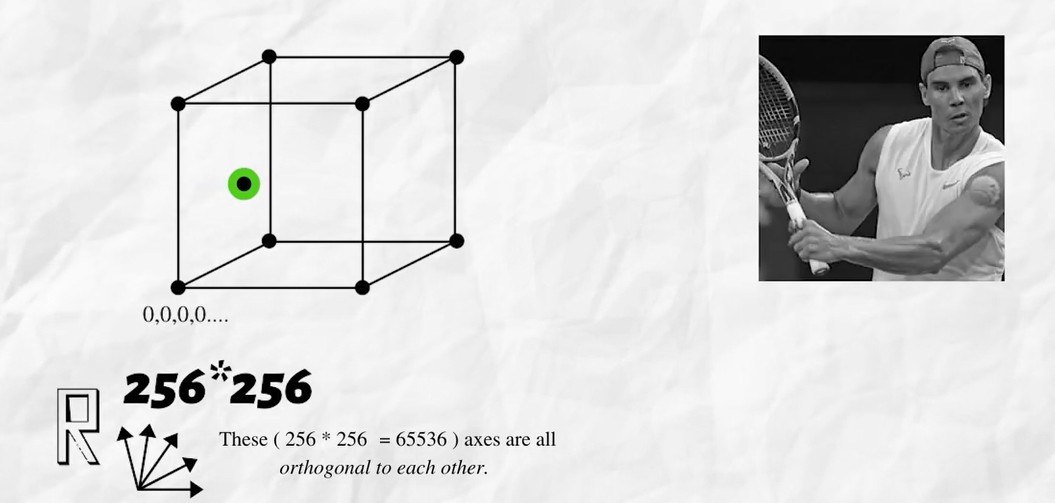
\includegraphics[width=0.5\linewidth,keepaspectratio]{gdl19}

{\tiny (Ref: My Understanding of the Manifold Hypothesis - Kartik Chincholikar)}	

\end{center}	
\end{frame}

%%%%%%%%%%%%%%%%%%%%%%%%%%%%%%%%%%%%%%%%%%%%%%%%%%%%%%%%%%%
\begin{frame}[fragile]\frametitle{Transition Between Images}
    \begin{itemize}
        \item Linear interpolation between points (images) is often not smooth. That gives wierd images.
        \item Intermediate points may not resemble real faces.
        \item Smooth transitions exist along special curved paths, where all are valid images.
        \item These paths lie on the image manifold. E.g. path between morphing from smiling face  to a non-smiling face. Intermediate points are also valid faces.
    \end{itemize}
	
\begin{center}
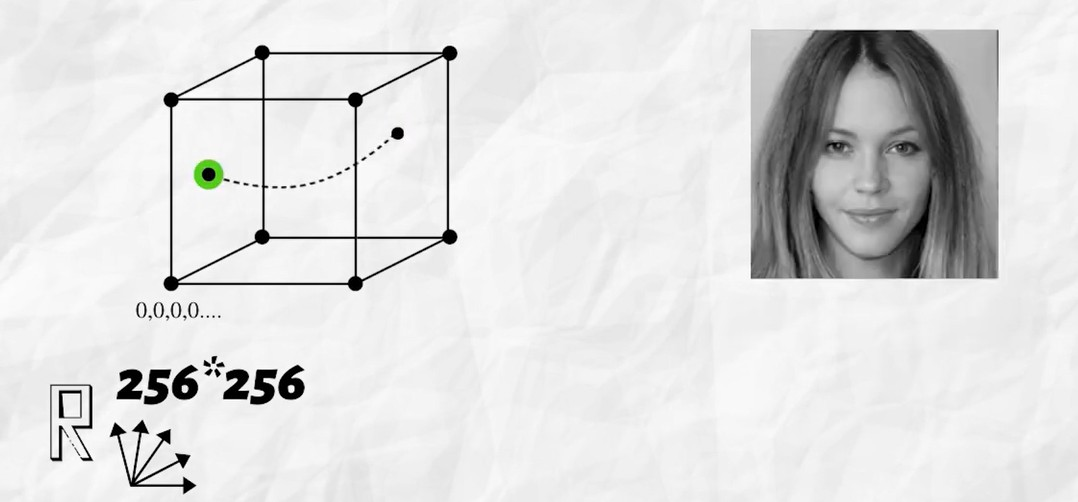
\includegraphics[width=0.5\linewidth,keepaspectratio]{gdl20}

{\tiny (Ref: My Understanding of the Manifold Hypothesis - Kartik Chincholikar)}	

\end{center}	


\end{frame}

%%%%%%%%%%%%%%%%%%%%%%%%%%%%%%%%%%%%%%%%%%%%%%%%%%%%%%%%%%%
\begin{frame}[fragile]\frametitle{Understanding the Face Manifold}
    \begin{itemize}
        \item Each realistic face image lies on or near a manifold.
        \item Moving on the manifold changes expressions smoothly.
        \item Moving off the manifold leads to unrealistic images.
        \item Faces = low-dimensional structure in high-dimensional space, aka Parametric Space that's one dimensional manifold versus 2 dimensional Model or Image space.
    \end{itemize}
	
\begin{center}
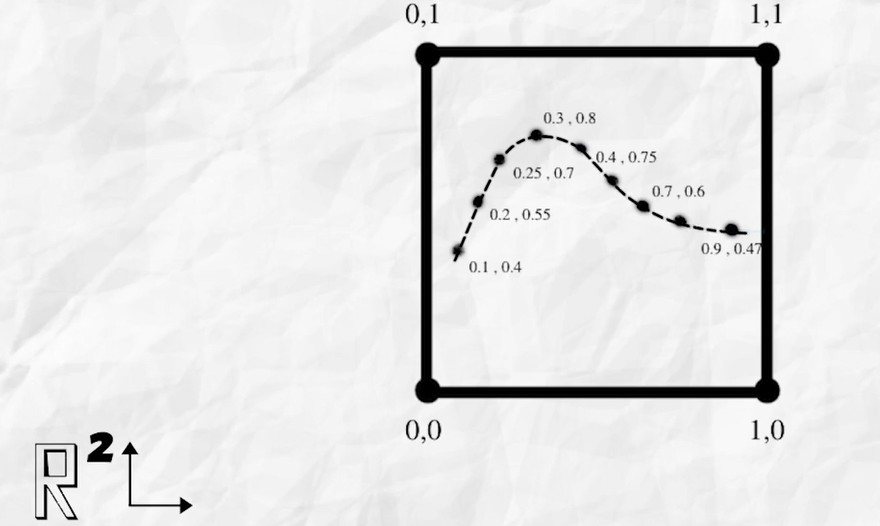
\includegraphics[width=0.5\linewidth,keepaspectratio]{gdl21}

{\tiny (Ref: My Understanding of the Manifold Hypothesis - Kartik Chincholikar)}	

\end{center}		
\end{frame}

%%%%%%%%%%%%%%%%%%%%%%%%%%%%%%%%%%%%%%%%%%%%%%%%%%%%%%%%%%%
\begin{frame}[fragile]\frametitle{Manifolds in Ambient Space}
    \begin{itemize}
        \item Data may lie on a 1D manifold in a 2D space. Underlying geometry.
        \item Example: points following a curved line.
        \item Manifolds are homeomorphic to lower-dimensional Euclidean space.
        \item Local coordinates suffice for representation. Rest of the data is all noise.
    \end{itemize}
	
\begin{center}
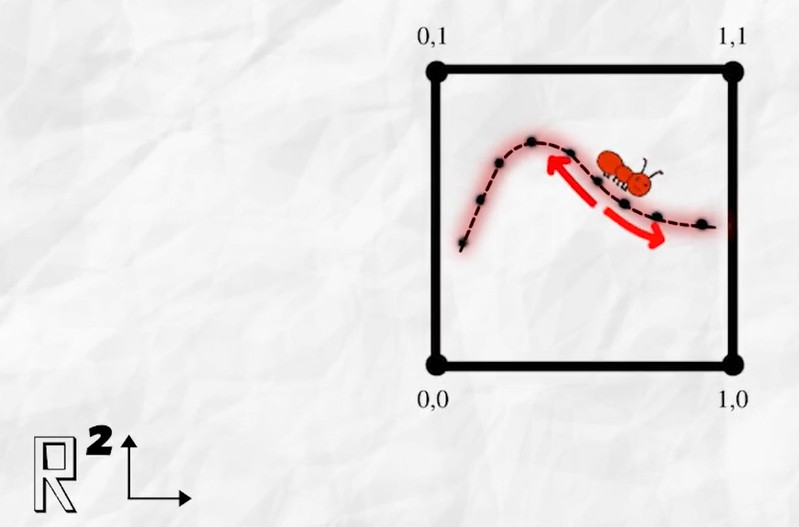
\includegraphics[width=0.5\linewidth,keepaspectratio]{gdl22}

{\tiny (Ref: My Understanding of the Manifold Hypothesis - Kartik Chincholikar)}	

\end{center}
\end{frame}

%%%%%%%%%%%%%%%%%%%%%%%%%%%%%%%%%%%%%%%%%%%%%%%%%%%%%%%%%%%
\begin{frame}[fragile]\frametitle{Degrees of Freedom and Natural Data}
    \begin{itemize}
        \item Real-world data has constraints: limited degrees of freedom.
        \item Example: height vs. weight correlation in humans.
        \item Physical laws restrict images: no cubic planets or levitating people.
        \item Natural images cluster on specific manifolds.
    \end{itemize}
	
\begin{center}
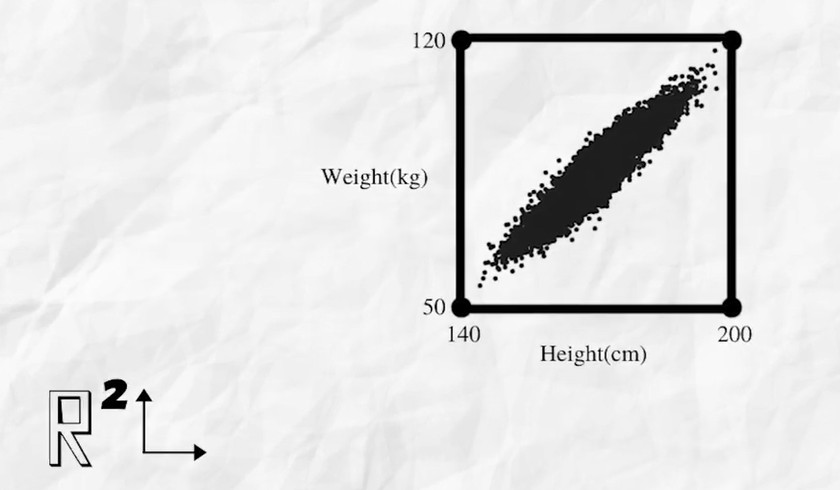
\includegraphics[width=0.5\linewidth,keepaspectratio]{gdl23}

{\tiny (Ref: My Understanding of the Manifold Hypothesis - Kartik Chincholikar)}	

\end{center}	
\end{frame}

%%%%%%%%%%%%%%%%%%%%%%%%%%%%%%%%%%%%%%%%%%%%%%%%%%%%%%%%%%%
\begin{frame}[fragile]\frametitle{Exploring Manifolds Visually}
    \begin{itemize}
        \item Moving on a manifold preserves realistic image features.
        \item Deviating from the manifold introduces noise or anomalies.
        \item Clock images example: midpoints on/off manifold differ significantly.
        \item On-manifold interpolation leads to plausible results.
    \end{itemize}
	
\begin{center}
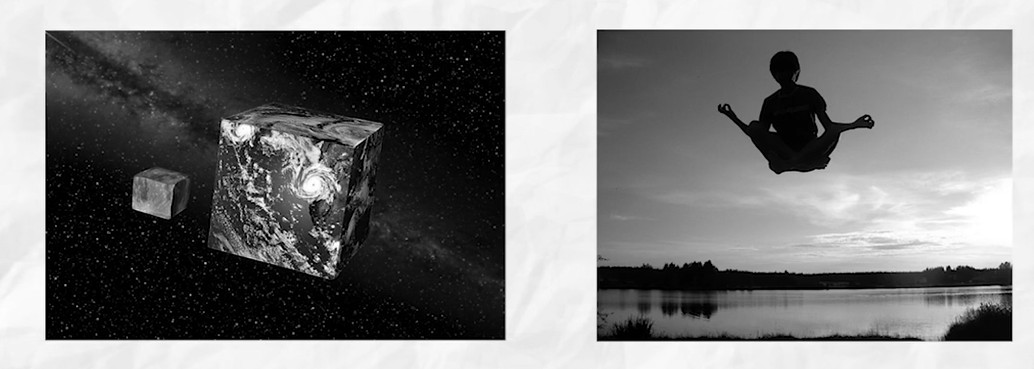
\includegraphics[width=0.7\linewidth,keepaspectratio]{gdl24}

{\tiny (Ref: My Understanding of the Manifold Hypothesis - Kartik Chincholikar)}	

\end{center}		
\end{frame}

%%%%%%%%%%%%%%%%%%%%%%%%%%%%%%%%%%%%%%%%%%%%%%%%%%%%%%%%%%%
\begin{frame}[fragile]\frametitle{Learning the Manifold}
    \begin{itemize}
        \item ML models aim to approximate data manifolds.
        \item VAEs and GANs learn mappings from latent to pixel space.
        \item Latent space is low-dimensional, manifold is high-dimensional.
        \item Models learn this mapping via optimization, not manual rules.
    \end{itemize}
	
\begin{center}
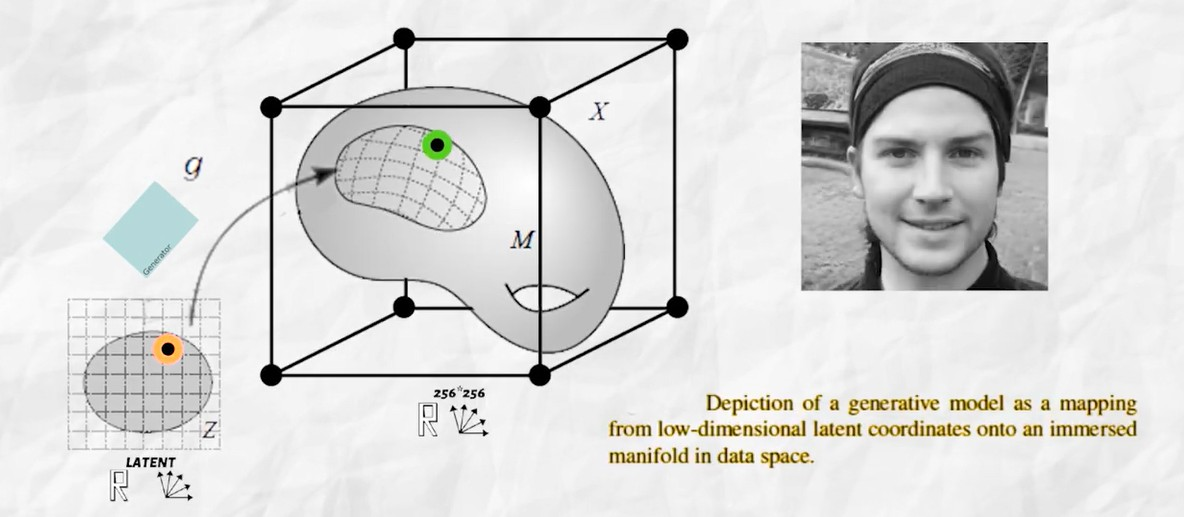
\includegraphics[width=0.5\linewidth,keepaspectratio]{gdl25}

{\tiny (Ref: My Understanding of the Manifold Hypothesis - Kartik Chincholikar)}	

\end{center}	
\end{frame}

%%%%%%%%%%%%%%%%%%%%%%%%%%%%%%%%%%%%%%%%%%%%%%%%%%%%%%%%%%%
\begin{frame}[fragile]\frametitle{Control and Future Directions}
    \begin{itemize}
        \item Better control of latent features is an active research area.
        \item Goal: steer generation with interpretable latent directions.
        \item Understanding manifolds improves generative model performance.
    \end{itemize}
\end{frame}
